Le système que nous proposons dans le présent document possédera des services accessibles depuis l'extérieur, et que nous pouvons visualiser à la figure \ref{famille}. Parmi ces
fonctionnalités, certaines seront dédiées à la famille des patients. Ces services auraient, bien entendu, un contrôle d'accès très
strict. Une possibilité que nous avons envisagée est l'envoie d'un sms aux numéros à prévenir en cas d'urgence d'un patient. Ce
sms contiendrait un mot de passe et un identifiant valides que durant la période d'hospitalisation. Le destinataire pourrait alors
se connecter à un site web (via une connexion sécurisée) où il pourrait trouver différentes informations et différents conseils.
\newline
\begin{figure}[h!]
	\hspace*{-2.5cm}
	\centering
	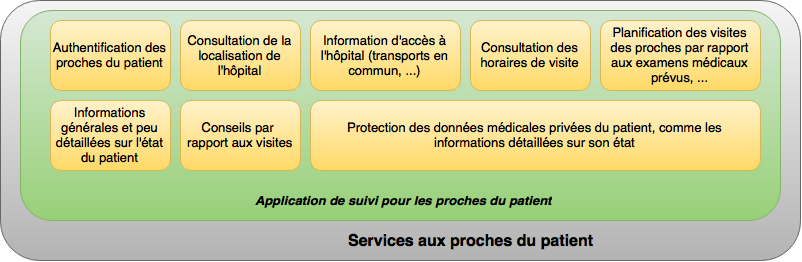
\includegraphics[width=1.4\textwidth]{famille.png}
	\caption{Services de la Couche Applicative du côté des Proches du Patient}
	\label{famille}
\end{figure}

Les informations visibles seraient la localisation de l'hôpital, comment s'y rendre ainsi que la chambre du patient. On pourrait
ajouter à cela les horaires des visites. Si l'on désire pousser cette idée plus loin, on peut imaginer un système où la famille
pourrait prendre rendez-vous sur un calendrier. S'il y a trop de visiteurs sur la période choisie, la demande de visite sera
refusée et l'utilisateur sera invité à choisir un autre moment. Ce système permettrait de mieux étaler les visites, évitant ainsi
que le patient ait trop de visiteurs à un certain moment, et aucun à d'autres moments. Cela permettrait aussi d'éviter que des
visiteurs viennent à une période où une opération est prévue. Ce qui les obligerait à rebrousser chemin. En revanche, les
informations médicales sensibles du patient ne seraient pas affichées, d'une part pour éviter une certaine atteinte à la vie
privée, et d'autre part pour limiter les mouvements de panique du côté des utilisateurs. Toutefois les informations médicales
utiles à la famille seraient accessibles. Cela permet d'empêcher que le service téléphonique de l'hôpital soit  surchargé par des
appels de proches exigeant des nouvelles.De manière générale, les consignes à respecter lors d'une visite seraient visibles sur
ce site. Et certaines informations sans lien direct avec l'hôpital mais utiles pour le confort des patients pourraient être
ajoutées. Connaître l'adresse de l'hôtel (ou équivalent) le plus proche serait, par exemple, un plus pour les visiteurs.
\newline

En plus des informations citées plus haut, nous aurions également des conseils à l'intention des personnes qui rendent visite aux
patients. Ces conseils pourraient être personnalisés selon le patient. A titre d'exemple, si leur traitement leur interdit un certain type d'aliments
cela serait précisé. 
\newline

Pour conclure cette partie, on notera qu'un tel système permettrait de réduire la charge du service public de l'hôpital, car de
nombreuses responsabilités qui étaient auparavant à leur charge seraient maintenant remplies par le site internet. De plus, il permettrait
d'améliorer l'expérience du visiteur en lui fournissant des informations et services utiles et disponibles à toutes heures.
Précisons que ce service devrait tourner sur le cloud public de l'hôpital.
\newline

Les services présentés ne peuvent être efficaces en l'absence de certains requis, qu'il convient de présenter.
\begin{enumerate}
    \item disponible : une forte disponibilité n'est pas requise, mais si le site discuté plus haut n'est pas accessible alors les
    responsabilités qui assuraient seraient de nouveau à la charge du personnel.
    \item Fiable : pour les mêmes raisons que précédemment. De plus, il doit également être fiable dans le sens commun du terme.
    En effet, si les informations présentées ne sont pas véridiques, l'hôpital perd en crédibilité. Et il risque de subir la
    colère et l'inquiétude des proches.
    \item sécurité : les communications doivent commencer par une phase d'authentification et être toujours chiffrées.
 \end{enumerate}
